\documentclass{beamer}

\usepackage[UTF8,noindent]{ctexcap}
\usepackage{color}%引入颜色
\usetheme{Copenhagen}%使用Copenhagen主题
\usepackage{graphicx}%引入插图
\usepackage{ulem}%删除线
\usepackage{tikz}
\usepackage{amsmath}
\usefonttheme[onlymath]{serif}

\title{决策单调性与四边形不等式}
\author{长郡中学\ \ 彭思进}
\date{2021 年 5 月 19 日}
\begin{document}
\begin{frame}
\titlepage
\end{frame}
\section{前言}
\subsection{前置定义与约定}
\begin{frame}{前置定义与约定}
	若无特殊说明,本文中提到的所有数取值范围为 $R^+ \cup \{+\infty\}$,其中 $\forall x \in R^+, x < +\infty,(+\infty)\pm x = +\infty$,某个元素等于正无穷常常表示这个元素不合法或不能被选取。
	
	对于 $n \times m$ 的矩阵 $A$,定义 
	\begin{itemize}
		\item 子矩阵 $A_{[i_1,\cdots,i_k],[j_1,\cdots,j_l]}$ 为矩阵 $A$ 的第 $i_1,i_2,\cdots,i_k$ 行和第 $j_1,\cdots,j_l$ 列的交集组成的矩阵;
		\item 连续子矩阵 $A_{[i_1 \sim i_2],[j_1 \sim j_2]} = A_{[i_1,i_1+1,\cdots,i_2],[j_1,j_1+1,\cdots,j_2]}$;
		\item $\min_i(A)$ 为最大的整数 $k$ 满足 $\forall 1 \leq j \leq m, A_{i,j} \geq A_{i,k}$。
	\end{itemize}

	为了避免输入成为瓶颈,下文除了特殊说明认为所有初始给出的矩阵中元素可以以较快的预处理和单次计算复杂度内得到,而不是完全依赖输入。
\end{frame}
\subsection{简介}
\begin{frame}{单调矩阵}
	\begin{definition}[单调矩阵]
		对于 $n \times m$ 的矩阵 $A$,若 $\forall 1 \leq i < j \leq n, \min_i(A) \leq \min_j(A)$,则称该矩阵为\textbf{单调矩阵(monotone matrix)}。
	\end{definition}
	\begin{definition}[完全单调矩阵]
		对于 $n \times m$ 的矩阵 $A$,若其所有子矩阵均是单调矩阵,则称 $A$ 为\textbf{完全单调矩阵(totally monotone matrix)}。
	\end{definition}
	大家常说的决策单调性问题均可转化为单调矩阵或完全单调矩阵上求解行最小值的问题。这类问题有复杂度远小于矩阵中元素个数的算法。
\end{frame}
\begin{frame}{四边形不等式}
	\begin{definition}[四边形不等式]
		对于 $n \times m$ 的矩阵 $A$,若对任意 $1 \leq i_1 \leq i_2 \leq n, 1 \leq j_1 \leq j_2 \leq m$ 均有 $A_{i_1,j_1} + A_{i_2,j_2} \leq A_{i_1,j_2}+A_{i_2,j_1}$,则称 $A$ 满足\textbf{四边形不等式(quadrangle inequality)},亦称矩阵 $A$ 为\textbf{蒙日阵(monge matrix)}。
	\end{definition}
	根据定义判定某个矩阵是否满足四边形不等式是 $O(n^2m^2)$ 的,但根据以下结论可以 $O(nm)$ 进行判定:
	\begin{theorem}[四边形不等式判定]
		$n \times m$ 的矩阵 $A$ 满足四边形不等式当且仅当对于任意 $1 \leq i < n, 1 \leq j < m, A_{i,j} + A_{i+1,j+1} \leq A_{i+1,j}+A_{i,j+1}$。
	\end{theorem}
\end{frame}
\begin{frame}{为什么选择四边形不等式?}
	\begin{theorem}
		若矩阵 $A$ 满足四边形不等式,则 $A$ 和 $A^T$ 是完全单调矩阵。
	\end{theorem}
	
	我们常常可以\sout{在打表之外}通过证明矩阵满足四边形不等式得出其满足完全单调矩阵的性质,通过行或列的单调性优化问题。同时蒙日阵还有以下显然但重要的性质使得其拓展性非常强:
	
	\begin{lemma}[]
		若矩阵 $A$ 满足四边形不等式,则给其任意一行或任意一列加上任意一个常数 $c$,其仍满足四边形不等式。
	\end{lemma}
\end{frame}
\begin{frame}{四边形不等式在动态规划中的应用举例 1}
考虑以下规模为 $n \times m$ 的动态规划(忽略初始值) $$f_{i,j} = \min_{1 \leq k < j} f_{i-1,k} + w_{k,j}$$用 $f_{i-1}$ 转移到 $f_i$ 时可以构造这样一个 $n \times n$ 的矩阵 $A$ 满足 $$ A_{x,y} = \begin{cases}
f_{i-1,y} + w_{y,x}, & x>y\\
\infty, & x \leq y
\end{cases} $$

那么 $f_{i,x} = A_{x,\min_x(A)}$。当矩阵 $W$ 满足元素可快速计算和四边形不等式时则可以使用马上将要提到的一系列方法。
\end{frame}
\begin{frame}{四边形不等式在动态规划中的应用举例 2}
	另一个规模为 $n$ 的动态规划长这样 $$f_i= \min_{1 \leq j < i} f_i + w_{j,i}$$ 类似地可以构造矩阵 $A$:$$ A_{x,y} = \begin{cases}
	f_{y} + w_{y,x}, & x>y\\
	\infty, & x \leq y
	\end{cases} $$
	当矩阵 $W$ 满足元素可快速计算和四边形不等式时仍然有决策单调性,但比较毒瘤的地方是计算 $f_i$ 时必须要求 $f_{1 \sim i-1}$ 均计算完成,这使得部分算法无法应用在这种情况上。
	
	为了区分两种情况,我们暂称举例 2 的情况为在线决策单调性,而举例 1 的情况为离线决策单调性。
\end{frame}
\section{决策单调性的决策点计算}
\subsection{分治}
\begin{frame}{分治}
	决策单调性问题最简单的解决算法是分治法。定义分治过程 $\texttt{solve(l,r,L,R)}$ 为计算 $l$ 到 $r$ 行最小值所在列,且已知它们的最小值所在列在 $L$ 至 $R$ 列。算法流程如下。
	\begin{enumerate}
		\item 若 $l>r$ 结束该过程;
		\item 设 $mid = \lfloor \frac{l+r}{2} \rfloor$,暴力枚举 $[L,R]$ 计算 $M=\min_{mid}(A)$;
		\item 递归 $\texttt{solve(l,mid-1,L,M)}$ 和 $\texttt{solve(mid+1,r,M,R)}$。
	\end{enumerate}\pause
	每次分治的复杂度是 $O(R-L)$。分治树上每层的复杂度总和不超过 $O(m)$,因此复杂度为 $O(m \log n + n)$。可以证明\textbf{单调矩阵}行最小值计算复杂度下界是 $O(m \log n)$。
	
	分治的一个很明显的缺点是无法解决在线问题,因为计算 $\min_{mid}(A)$ 时 $\min_{l \sim mid-1}(A)$ 未算出。但相比于后面的二分栈与 SMAWK 算法来说,其又有一个独特的性质,下举一例。
\end{frame}
\begin{frame}{例题 1:小 Z 的游览计划}
Source:北大集训 2018 Day3 T3

给出 $n$ 个点的树和一个 $1 \sim n$ 的排列 $p$。要求将排列分成连续非空
的 $k$ 段区间。定义一段区间的价值为区间内所有点并上 $1$ 在给出树上的最小斯坦纳树边数和。求所有划分方案中最大权值和。

$n \times k \leq 2 \times 10^5$
\end{frame}
\begin{frame}{例题 1 解决思路——四边形不等式}
设 $val_{i,j}$ 表示区间 $[i,j]$ 的价值,则对于任意 $1 \leq i < j \leq n$ 有 $val_{i,j}+val_{i+1,j+1} \geq val_{i,j+1}+val_{i+1,j}$。权值取负之后就变成最开始提到的离线决策单调性,但一个重要的问题是 $val_{i,j}$ 无法 $O(1)$ 计算。\pause

一个重要的观察是:用 set 维护了 $p_i,p_{i+1},\cdots,p_j$ 的 dfs 序和 $val_{i,j}$ 之后,可以在 $O(\log n)$ 的时间内计算 $val_{i,j-1},val_{i,j+1},val_{i+1,j},val_{i-1,j}$ 的取值。这样的性质下使用分治算法会有很大的优势。
\end{frame}
\begin{frame}{例题 1 解决思路——分治算法}
分治算法的流程与上面无异,只是在权值计算上有所差别:单独维护两个指针 $i,j$ 并维护 $val_{i,j}$ 的取值以及 $\{p_i,\cdots,p_j\}$ 点集的 dfs 序 set。每次询问 $val_{x,y}$ 的时候暴力移动指针 $i,j$ 的取值并更新 $val_{i,j}$,当 $i=x$ 且 $j=y$ 时返回答案。\pause

考虑分析指针移动的次数。对于分治过程 \texttt{solve(l,r,L,R)},考虑这个分治节点产生的复杂度,分为这几个部分:
\begin{enumerate}
\item 计算 $mid$ 的最优转移;
\item 将指针移动到左分治区间的第一次询问所在位置;
\item 将指针移动到右分治区间的第一次询问所在位置;
\end{enumerate}
注意左右区间各自的计算流程不算在当前\textbf{节点}的计算复杂度内。可以发现这三者的复杂度都不超过 $O(r-l+R-L)$,因此总移动次数是 $O((n+m)\log n)$ 的。算上 set 的复杂度,在本题中运用这个算法复杂度即为 $O(kn\log^2 n)$。
\end{frame}
\subsection{二分栈}
\begin{frame}{完全单调矩阵的性质}
	在介绍二分栈以及之后的 SMAWK 算法前先说明若干性质,这些性质通过完全单调矩阵和单调矩阵的定义可以立即得出:
	\begin{enumerate}
		\item 对于 $n \times m$ 的完全单调矩阵 $A$ 和 $1 \leq i < j \leq m$,存在整数 $0 \leq p_{i,j} \leq n$ 使得对于任意 $1 \leq k \leq n$,$A_{k,i} < A_{k,j}$ 当且仅当 $k \leq p_{i,j}$;
		\item 对于 $n \times m$ 的完全单调矩阵 $A$ 定义某个元素是冗余的当且仅当其不是对应行的最小值所在位置,若 $A_{k,i} < A_{k,j}$,则 $A_{1,j},A_{2,j},\cdots,A_{k,j}$ 都是冗余的,否则 $A_{k,i},A_{k+1,i},\cdots,A_{n,i}$ 都是冗余的。定义某一列是冗余的当且仅当其所有元素都是冗余的。
	\end{enumerate}
\end{frame}
\begin{frame}{二分栈算法}
	二分栈算法是增量算法,可以解决在线情况。其按顺序加入每一列,用栈维护矩阵中不是冗余列的列,维护它们在哪些行上作为最小值列。由于单调性,若第 $j$ 列不是冗余的,则有某个行区间 $[l_j,r_j]$ 以第 $j$ 列作为最小值所在列。加入第 $i$ 列时,会有行的一段后缀以第 $i$ 列作为最小值列,计算这个后缀并维护栈的算法流程如下:
	\begin{enumerate}
		\item 若栈空,则当前所有行都以该列作为最小值列,将 $i$ 入栈,$l_i \leftarrow 1, r_i \leftarrow n$,结束。
		\item 否则取栈顶元素 $j$。若 $A_{l_j,j} \geq A_{l_j,i}$,则第 $j$ 列的所有元素都是冗余的,弹栈并返回步骤 1;
		\item 否则二分计算 $t = p_{j,i}$,$r_j \leftarrow t$。若 $t \neq n$,将 $i$ 入栈,$l_i \leftarrow t + 1,r_i \leftarrow n$。
	\end{enumerate}
	加入所有列后即得最小值列分布。每列只会入出栈一次,仅有入栈进行一次二分,复杂度 $O(m \log n)$。
\end{frame}
\subsection{SMAWK}
\begin{frame}{SMAWK 算法简介}
	分治和二分栈算法是常见的解决决策单调性的算法,但复杂度都是 $O(m \log n)$。那么能否更进一步呢?
	
	首次提出完全单调矩阵的线性求解行最小值算法的是 Shor、Moran、Aggarwal、Wilber、Klawe 五位学者,因此之后大家以五个学者的姓首字母作为该算法名字,也就是 SMAWK 算法。
	
	SMAWK 算法只适用于离线情况,没有类似分治算法的移动指针性质,但只需要计算 $O(n+m(1+ \max(0,\log \frac{n}{m})))$ 个元素的取值以得到每行的最小值。
	
	例题:CF1423M 
\end{frame}
\begin{frame}{子过程 reduce}
	求解行最小值的矩阵行数少而列数多时,有很多列冗余,删除它们对答案不产生影响。故考虑子过程 $\texttt{reduce(A)}$,$A$ 是 $n \times m$ 的完全单调矩阵。其返回一个 $n \times \min(n,m)$ 的矩阵,结果为 $A$ 删除若干冗余的列得到的矩阵。其算法流程如下:
	\begin{enumerate}
		\item 初始定义 $k = 1$;
		\item 当 $n \geq m$ 时结束过程;否则比较 $A_{k,k}$ 和 $A_{k,k+1}$。
		\item 若 $A_{k,k} \geq A_{k,k+1}$,删除第 $k$ 列,$k \leftarrow \max(k-1,1)$,回到步骤 2;
		\item 若 $A_{k,k} < A_{k,k+1}$ 且 $k=n$,删除第 $n+1$ 列,回到步骤 2;
		\item 若 $A_{k,k} < A_{k,k+1}$ 且 $k \neq n$,$k \leftarrow k+1$,回到步骤 2。
	\end{enumerate}
\end{frame}
\begin{frame}{reduce 的复杂度和实现}
	reduce 过程会删除 $m-n$ 列,$k$ 的最大值为 $n$,而每次比较会导致 $k$ 减一并删除列数加一,或者 $k$ 加一,所以复杂度为 $O(m+n)$。
	
	直接暴力实现矩阵的任意列删除复杂度是不能接受的,因此实现时可以用链表维护未被删除的列编号,在链表上进行删除和维护前驱后继,这样可以 $O(1)$ 删除列。
\end{frame}
\begin{frame}{SMAWK 算法流程}
	SMAWK 算法是一个递归算法,借用 reduce 作为子过程。过程 $\texttt{SMAWK(A)}$ 表示计算 $n \times m$ 的完全单调矩阵 $A$ 的每行最小值所在列。算法流程如下:
	\begin{enumerate}
		\item 若 $\min(n,m) = 1$ 直接计算答案;
		\item 设 $B = \texttt{reduce(A)},C = B_{[2,4,\cdots,2\lfloor \frac{n}{2} \rfloor] , [1,2,\cdots,\min(n,m)]}$;
		\item 递归计算 $\texttt{reduce(C)}$ 得到偶数行最小值所在列;
		\item 对于 $B$ 中的奇数行,在其相邻两行的最小值所在列之间暴力枚举计算出其最小值所在列。
	\end{enumerate}
	由于有相邻两行的限制,步骤 4 复杂度 $O(m)$。需要注意由于在递归过程中删除了若干中间的列,所以回溯的时候要注意列编号的维护。
\end{frame}
\begin{frame}{SMAWK 的复杂度和实现}
	设 $f(n,m)$ 表示 $n \times m$ 的矩阵作为 SMAWK 算法参数时的复杂度,在 $m \geq n$ 时有递归式 $f(n,m) = f(\frac{n}{2} , n) + O(m+n)$,可以解出 $f(n,m) = O(m+n)$。$n > m$ 时 $f(n,m) = f(\frac{n}{2} , m) + O(m+n)$,递归 $\log \frac{n}{m}$ 层之后进入 $n \leq m$ 的情况,所以复杂度为 $O(m(1 + \log \frac{n}{m}) + n)$。
	
	具体实现的时候需要快速提取矩阵 $A$ 的子矩阵,可以使用链表维护该子矩阵在原矩阵上的行编号和列编号表示子矩阵保证复杂度正确。
\end{frame}
\begin{frame}{还想要更多……}
	SMAWK 算法只能计算离线问题不够优秀。在本部分后面,通过拓展 SMAWK 算法,得到了两个线性的决策单调性算法,其中 Wilber 算法可以解决部分在线决策单调性问题,而 Eppstein 和二分栈算法的能力相同,且复杂度均为 $O(n)$。
	
	但因为其常数比较大且时间有限不进行赘述。
\end{frame}
\subsection{*Wilber}
\begin{frame}{Wilber 算法}
	SMAWK 算法的一个显著劣势是无法处理在线情况。那么形如 $f_i = \max_{1 \leq i < j} f_j + w_{j,i}$ 的动态求解行最小值能否做到线性的复杂度?
	
	以 SMAWK 算法作为子过程,Wilber 发明了一个新算法,以线性的复杂度解决上面这类动态规划对应的矩阵行最小值问题。
\end{frame}
\begin{frame}{Wilber 算法流程}
	为了方便认为权值矩阵 $A$ 是 $n \times n$ 的方阵。
	\begin{enumerate}
		\item 初始定义 $r=c=1$。算法中满足 $1 \leq r \leq c \leq n$,$f_1 \sim f_c$ 已经确定,且 $f_{c+1}$ 的转移点至少是 $r$。$c=n$ 时算法结束;
		\item 定义 $p = \min(n,c+(c-r+1))$,用 SMAWK 计算 $A_{[c+1 \sim p],[r \sim c]}$ 中行最小值作为 $f$ 的估计值,记作 $g_{c+1 \sim p}$,;
		\item 考虑 $(p-c) \times (p-c)$ 的矩阵 $B$,$B_{i,j} = \begin{cases}
		+\infty, & i \leq j \\
		g_{j+c} + w_{j+c,i+c}, & i > j
		\end{cases}$,用 SMAWK 计算其行最小值,记作 $h_{c+1 \sim p}$,也就是用 $g$ 转移做二次估计。
	\end{enumerate}
\end{frame}
\begin{frame}{Wilber 算法流程——续}
\begin{enumerate}\setcounter{enumi}{3}
	\item 若对于所有 $c+1 \leq i \leq p$ 都有 $g_i \leq h_i$,那么 $g$ 作为 $f$ 的估计值均是正确的,$\forall c+1 \leq i \leq p, f_i \leftarrow g_i$,然后 $c \leftarrow p$,回到步骤 2;
	\item 否则找到最小的整数 $t$ 使得 $g_t > h_t$,那么 $c+1 \sim t-1$ 部分 $g$ 的估计正确,$t$ 位置 $h$ 的估计正确且转移点至少是 $c+1$,$t$ 以后的以已经算出的部分不能确定答案。此时 $\forall c+1 \leq i \leq t-1,f_i \leftarrow g_i$,$f_t \leftarrow h_t, r \leftarrow c+1,c \leftarrow t$,回到步骤 2。
\end{enumerate}
算法的正确性还是很容易理解的。下面来简要说明一下其复杂度。
\end{frame}
\begin{frame}{Wilber 算法复杂度分析}
	称做一轮 234/235 操作为一轮操作。首先最后一轮操作完成后有 $c=n$,这一轮的复杂度是 $O(n)$。
	
	对于其他轮的操作,步骤 2,3 的复杂度均为 $O(c-r)$。此时若进入步骤 4,则 $c$ 会增加 $p-c = c-r$;若进入步骤 5,则 $r$ 会增加 $c-r$。因此 $r+c$ 的增加量至少是 $c-r$,可以看作 $r+c$ 每增加 $1$ 付出均摊 $O(1)$ 时间;而 $r+c \leq 2n$ 所以复杂度是均摊 $O(n)$。\pause
	
	看起来我们获得了一个能够完全替代二分栈的动态求行最小值的线性算法。可真的是这样吗?
\end{frame}
\subsection{*Eppstein}
\begin{frame}{问题引入——交错动态规划}
	我们可以考虑这样的一个动态规划:
	\begin{gather*}
		f_i = \min_{1 \leq j < i} g_j + w_{j,i} \\
		g_i = \min_{1 \leq j < i} f_j + w'_{j,i}
	\end{gather*}
	其中 $w_{j,i},w'_{j,i}$ 构成的权值矩阵满足四边形不等式。我们可以称其为交错动态规划,原因是其中的某个动态规划的转移受到其他动态规划的前驱值影响,而其他的动态规划的前驱取值又受到该动态规划的前驱值影响。
	
	二分栈算法可以容易地解决这样的动态规划,那么直接拓展 Wilber 算法是否可以在线性复杂度内完成计算呢?
\end{frame}
\begin{frame}{Wilber 算法在交错动态规划上的直接拓展尝试}
	考虑同时进行两个动态规划的 Wilber 算法,也就是将它们的每个步骤都放在一起运行。此时会出现一些问题。
	
	不妨假设当前算法第一次出现二次估计值是正确值的位置是 $t$,而其中仅有 $f_t$ 的值是第二估计值,而 $g_t$ 的值是第一估计值。此时已确定的前缀数量 $c \leftarrow t$,但对于 $g$ 的动态规划来说,无法保证 $g_t$ 的转移点在 $r$ 之后,所以不能移左端点,均摊的复杂度分析遭到破坏。\pause
	
	Wilber 算法看起来并不能直接使用。此时 Eppstein 对 Wilber 提出的算法进行了一些修改,使得其可以解决更加强的交错动态规划的情况并保持线性复杂度,运用情景基本比肩二分栈算法。
	
\end{frame}
\begin{frame}{Eppstein 算法}
	设使用该算法维护的 dp 是 $f$,转移依赖数组 $g$,权值矩阵 $A$ 是 $n \times n$ 的方阵。仍然维护 $r,c$,初始 $r = c = 1$,其中 $f_{1 \sim c}$ 和 $g_{1 \sim c}$ 均已算出,维护 $E_1 \sim E_n$,满足 $f_i = \min(E_i , \min_{j \geq r} g_j+w_{j,i})$,也就是存 $<r$ 的所有转移中有意义的值。初始 $E_i = +\infty$。
	
	这个算法相比 Wilber 算法的优势在于其可以按照 $f_1,f_2,\cdots,f_n$ 的顺序一个个确定值,而不会如 Wilber 算法一次性求一个连续区间的取值。这样多个 Eppstein 算法交错转移也是允许的。
\end{frame}
\begin{frame}{Eppstein 算法流程}
	\begin{enumerate}
		\item 设 $p=\min(c+(c-r+1),n)$,对 $A_{[r \sim c],[c+1 \sim p]}$ 运行 SMAWK 计算 $f_{c+1 \sim p}$ 在 $\geq r$ 的转移点估计值,和 $E_{c+1 \sim p}$ 取最小值后得到真实估计值,记作 $h_{c+1 \sim p}$;
		\item 然后对 $i\in[c+1,p]$ 计算 $v_i = \max_{i < j \leq p} h_j-w_{i,j}$,也就是 $g_i$ 小到多少会破坏 $h$ 的估计。这是完全单调矩阵行最小值问题,SMAWK。设 $k=c$ 表示已经计算完的元素位置。
		\item $k \leftarrow k+1$ 并 $f_k \leftarrow h_k$ 表示新确定元素取值,然后计算 $g_k$。若 $k=p$,则这一轮计算完成,$c \leftarrow p$ 回到步骤 1;否则考察 $g_k$ 与 $v_k$ 的大小关系。
		\item 若 $g_k \geq v_k$ 则不会破坏估计,回到步骤 3;
		\item 否则 $\forall i\in[c+1,p],E_i \leftarrow h_i$,$r \leftarrow c+1$,$c \leftarrow k$,回到步骤 1。
	\end{enumerate}
\end{frame}
\begin{frame}{算法正确性简述和复杂度}
	复杂度计算是简单的,和 Wilber 算法一致,是 $O(n)$ 的。
	
	正确性上比较魔幻的是步骤 5。发现 $g_k<v_k$ 时,$> k$ 位置的估计可能发生错误。此时先把 $[c+1,p]$ 这部分内的 $E_i$ 进行更新,更新为 $\leq c$ 部分的转移贡献;而对于 $[p+1,n]$ 部分,注意到 $[c+1,p]$ 区间内已经存在一个转移点大于 $c$ 的位置了,所以后面这些位置的转移点也大于 $c$,不更新 $E$ 数组也可以得到正确结果。
	
	$E$ 数组存在的意义是进入步骤 5 只能知道 $[c+1,p]$ 区间内存在某个位置转移点大于 $c$,但 $[c+1,p]$ 区间内仍有部分转移点 $\leq c$ 的位置没有更新转移,所以用 $E$ 暂存这部分结果。
\end{frame}
\section{二维决策单调性}
\subsection{最优搜索树问题}
\begin{frame}{最优搜索树问题}
相信大家在入门区间 DP 时都做过一道叫做“石子合并”的题目,这个问题实际上是给出每个元素询问次数,要求建立一棵搜索树最小化查询时间和。该题目的动态规划大概是这个样子的:

$$f_{i,j} = \begin{cases}
0, &i \geq j \\
w_{i,j}+\min_{i \leq k < j} f_{i,k} + f_{k+1,j} &i<j
\end{cases}$$

当 $w_{i,j}$ 构成的权值矩阵满足四边形不等式,且对于 $i \leq i' \leq j' \leq j$ 有 $w_{i,j} \geq w_{i',j'}$(我们称这个性质为区间单调性)时,其亦可进行优化将复杂度从 $O(n^3)$ 降低。
\end{frame}
\subsection{朴素动态规划算法的加速}
\begin{frame}{答案矩阵的性质}
	\begin{theorem}
		矩阵 $\{f_{i,j}\}$ 满足四边形不等式,即对于 $i \leq i' \le j \leq j',f_{i,j}+f_{i',j'} \leq f_{i,j'}+f_{i',j}$。
	\end{theorem}\pause
	设 $f_{i,j,y}$ 表示从 $y$ 决策点转移 $f_{i,j}$ 的结果,即 $w_{i,j}+f_{i,y}+f_{y+1,j}$。对 $j'-i$ 归纳,$j'-i \leq 1$ 时有 $i=i'$ 或 $j=j'$ 显然成立。当结论对 $j'-i-1$ 成立时,讨论 $i' = j$ 是否成立。
	
	$i '= j$ 时,需要证明 $f_{i,j}+f_{j,j'} \leq f_{i,j'}$,称其为三角形不等式。假设 $f_{i,j'}$ 的最优取值转移点是 $y$,且 $y < j$,则
	\begin{equation*}
	\begin{split}
	f_{i,j} + f_{j,j'} &\leq f_{i,j,y}+f_{j,j'}= w_{i,j} + f_{i,y}+f_{y+1,j}+f_{j,j'} \\ & \leq w_{i,j'}+f_{i,y}+f_{y+1,j'} = f_{i,j',y}=f_{i,j'}
	\end{split}
	\end{equation*}
	$y \geq j$ 时拆 $f_{j,j'}$ 同理。
\end{frame}
\begin{frame}{答案矩阵的性质}
	当 $i' \neq j$ 时,设 $f_{i,j'}$ 和 $f_{i',j}$ 的最优转移点分别是 $y$ 和 $z$ 且 $y \leq z$。此时有
	\begin{equation*}
	\begin{split}
	f_{i,j} + f_{i',j'} & \leq f_{i,j,y} + f_{i',j',z} \\ 
	&=(w_{i,j}+w_{i',j'})+(f_{i,y}+f_{i',z})+(f_{y+1,j}+f_{z+1,j'}) \\ 
	&\leq(w_{i,j'}+w_{i',j})+(f_{i,y}+f_{i',z})+(f_{y+1,j'}+f_{z+1,j}) \\ &= f_{i,j',y}+f_{i',j,z} = f_{i,j'}+f_{i',j}
	\end{split}
	\end{equation*}
	$y>z$ 时类似。
\end{frame}
\begin{frame}{决策单调性}
	\begin{theorem}
		设 $f_{i,j}$ 最小的最优转移点为 $K_{i,j}$,则有 $K_{i-1,j} \leq K_{i,j} \leq K_{i,j+1}$。
	\end{theorem}\pause
	这里只证明 $K_{i,j} \leq K_{i,j+1}$,另一边是一样的。
	
	对于一个确定的 $i$,考虑 $n \times n$ 矩阵 $A$ 满足
	
	$$a_{p,q}= \begin{cases}
	w_{i,q} + f_{i,p}+f_{p+1,q},& i \leq p < q \\
	+\infty, & otherwise
	\end{cases}$$,则 $x_2,x_3,\cdots,x_{k+1},x_2+L$ 也是 $x_2 \rightarrow x_2 + L$ 字典序最小的最短路。
	
	则计算 $f_{i,q}$ 就是计算其第 $q$ 列最小值。由于矩阵 $\{f_{p,q}\}$ 是蒙日阵,故矩阵 $A$ 是蒙日阵,有 $K_{i,j} \leq K_{i,j+1}$。
\end{frame}
\begin{frame}{两维都单调的决策单调性计算}
	上面给出了结论描述了动态规划 $f$ 在两维上的单调性。利用该结论可以对动态规划的计算进行优化。
	
	设 $K_{i,i} = i$,按照区间长度顺序计算 $f$ 和 $K$。计算 $K_{i,j}$ 时,由于 $K_{i,j-1} \leq K_{i,j} \leq K_{i+1,j}$,故在 $K_{i,j-1}$ 和 $K_{i+1,j}$ 之间暴力枚举转移点。计算区间长度为 $L$ 的所有 $K$ 的复杂度为 $\sum_{i=1}^{n-L}(K_{i+1,i+L}-K_{i,i+L-1}) = K_{n-L,n-1} - K_{1,L+1} = O(n)$,总复杂度为 $O(n^2)$,常数较小。
\end{frame}
\subsection{*多叉树拓展}
\begin{frame}{多叉树拓展}
既然动态规划里可以分成两半,那么分成多个部分自然是可做的。对于寻找最优 $k$ 叉搜索树的区间动态规划 $$f_{i,j} = \begin{cases}
	0, & i \geq j\\
	w_{i,j}+\min_{i \leq p_1 \leq p_2 \leq \cdots \leq p_k < j} f_{i,p_1}+f_{p_1+1,p_2}+\cdots+f_{p_k+1,j}, &i<j
\end{cases}$$
论文 “Efficient Dynamic Programming Using Quadrangle Inequalities” 中给出了在权值矩阵满足四边形不等式、三角形不等式和区间单调性时将复杂度优化为 $O(n^2 \log k)$ 的算法。由于时间有限这里略去大部分证明仅给出算法流程,有兴趣的同学可自行阅读论文。

\sout{话说这玩意我好像还没有看到有人出过}
\end{frame}
\begin{frame}{多叉搜索树动态规划的优化}
	设下面三个动态规划式子,其中 $i>j$ 时值全部为 0。
	\begin{gather*}
	h^k_{i,j}=\min_{i \leq p_1 \leq p_2 \leq \cdots \leq p_k < j} f_{i,p_1}+f_{p_1+1,p_2}+\cdots+f_{p_k+1,j}\\
	h^{t}_{i,j} = \min_{i \leq p_1 \leq p_2 \leq \cdots \leq p_t \leq j} f_{i,p_1}+f_{p_1+1,p_2}+\cdots+f_{p_k+1,j}(1 < t < k) \\
	h^{1}_{i,j}=f_{i,j}
	\end{gather*}
	注意 $h^k$ 和 $h^t$ 选择下标的不同,$h^k$ 要求至少有两个非空区间,而 $h^t$ 只要求有一个。
\end{frame}
\begin{frame}{多叉搜索树动态规划的优化}
	对于 $r+s=t(t<k)$,可通过 $h^r$ 和 $h^s$ 得到 $h^t$:$$h^t_{i,j}=\min_{i\leq p\leq j}h^r_{i,p}+h^s_{p+1,j}$$ 对于 $r+s=k$ 也有类似式子 $$h^k_{i,j}=\min_{i\leq p< j}h^r_{i,p}+h^s_{p+1,j}$$
	可以对区间长度归纳证明 $h^t,h^k,f_{i,j}$ 矩阵均满足四边形不等式,两维上都具有决策单调性。
\end{frame}
\begin{frame}{多叉搜索树动态规划的优化}
	\begin{definition}[加法链]
		对整数 $k$ 认为一个序列 $p_1=1 < p_2<\cdots<p_l=k$ 是 $k$ 的\textbf{加法链(addition chain)}当且仅当对于每个 $x\in[2,l]$ 存在 $y,z \in [1,x-1],p_y+p_z=p_x$。
	\end{definition}
	对于任意整数 $k$ 显然存在长度为 $O(\log k)$ 的加法链 $p_1,\cdots,p_l$。枚举区间长度进行转移,对于 $x \in [2,l]$ 通过 $h^{p_y}$ 和 $h^{p_z}$ 计算 $h^{p_x}$,最后得到 $h^{k}$ 的取值即可得到 $f$ 取值。需要做 $O(\log k)$ 次二维决策单调性动态规划,复杂度为 $O(n^2 \log k)$。
\end{frame}
\section{决策单调性最短路问题}
\subsection{定义与基本算法}
\begin{frame}{决策单调性最短路问题}
	这个问题起源于从 DAG 最短路,问题是:给定 $n$ 个点的 DAG,点 $i$ 与点 $j$ 在 $i<j$ 时有边权值为 $w_{i,j}$。求 $1$ 到 $n$ 经过 $k$ 条边的最短路。
	
	将其描述为动态规划就是熟悉的形式:
	
	$$f_{i,j} = \min_{1 \leq k < j} f_{i-1,k} + w_{k,j}$$
	
	在权值矩阵 $W$ 满足四边形不等式时我们可以以 $O(nk)$ 的复杂度解决该问题。本节中我们探讨一些拓展和优化。
\end{frame}
\begin{frame}{例题 2:环上邮局}
	Source:\href{https://www.acmicpc.net/problem/18446}{XIX Open Cup named after E.V. Pankratiev. Grand Prix of Zhejiang I},可在 \href{https://acm.nflsoj.com/problem/216}{NFLSOJ216} 提交。
	
	在一个长度为正整数 $L$ 的环上的整点上有 $V$ 座村庄,你需要在环上修建 $P$ 个邮局,位置要求在整点,最小化每个村庄到距离其最近的邮局的距离和。按照不降顺序输出方案。
	
	$L \leq 10^{12}, 1 \leq P \leq V \leq 2.5 \times 10^5$,时间限制 5s
	
	Tips:dlsyyds
\end{frame}
\begin{frame}{例题 2 解法——基本转化}
	枚举每个位置,以该位置断环成链,转化为链上问题。链上问题最后一定是把村庄分成 $P$ 段,每段里的所有村庄选择同一个邮局。而一段中邮局选择村庄坐标中位数最优,前缀和后可 $O(1)$ 计算一段的权值。
	
	同时权值矩阵满足四边形不等式,由于时间关系略过证明。这样可得 $O(n^2k)$ 的做法。注意跑出来的结果是分成 $k$ 段的方案,还需要额外设置每段村庄的位置。
	
	下面我们将介绍如何将其优化至 $O(n^2 \log V)$、$O(n \log V+n^2)$ 和 $O(n \log V + n \log n)$,其中 $V$ 是答案上界。
\end{frame}
\subsection{答案凸性}
\begin{frame}{最短路问题与凸性}
	直接上定理。
	\begin{theorem}[答案凸性]
		设 $f(k)$ 表示该图中从 $1$ 到 $n$、经过 $k$ 条边的最短路,则 $f(k)$ 在定义域上是下凸函数,即 $\forall k \in [2,n-2]$,$f(k+1)-f(k) \geq f(k)-f(k-1)$。
	\end{theorem}
	求解下凸函数 $f(x)$ 在 $x=k$ 处的取值可以使用 wqs 二分完成。具体地,二分斜率 $mid$,求解该凸壳在 $mid$ 斜率处的切点,比较其与 $k$ 的大小关系进行调整。对应到最短路问题,求 $mid$ 斜率下最小值等价于权值矩阵全体减 $mid$ 后求解最小值,这可以用 Wilber 算法完成。这样定理中问题可以做到 $O(n^2 \log V)$。
\end{frame}
\begin{frame}{定理证明}
	背结论选手不要睡觉哦,这部分证明与方案构造有很大的关系。
	
	考虑证明以下引理:
	\begin{lemma}
		$\forall 1 \leq s < r < t \leq n-1,f(s)+f(t) \geq f(r)+f(s+t-r)$
	\end{lemma}
	该引理成立后代入 $s=k-1,r=k,t=k+1$ 即得 $f(k+1)-f(k) \geq f(k)-f(k-1)$,即原定理。
	
	证明引理前,设 $f(s)$ 对应的其中一个最优方案是 $p_1,p_2,\cdots,p_{s+1}$;$f(t)$ 对应的其中一个最优方案是 $q_1,q_2,\cdots,q_{t+1}$。
\end{frame}
\begin{frame}{引理证明}
	设 $v=r-s$,若找到 $i\in[1,s]$ 满足 $p_i \leq q_{i+v} < q_{i+v+1} \leq p_{i+1}$,则可构造路径 $p_1,\cdots,p_i,q_{i+v+1},\cdots,q_{t+1}$ 和 $q_1,\cdots,q_{i+v},p_{i+1},\cdots,p_{s+1}$,长度分别是 $s+t-r$ 和 $r$。由四边形不等式 $w_{p_i,q_{i+v+1}} + w_{q_{i+v},p_{i+1}} \leq w_{p_i,p_{i+1}} + w_{q_{i+v},q_{i+v+1}}$,所以 $f(s)+f(t)$ 不比这两条路径长度和小,即不比 $f(r)+f(s+t-r)$ 小。\pause
	
	~\\
	
	如何说明一定存在这样的 $i$?注意到 $q_{v+1} > 1$,考虑以 $p$ 作为分割点将 $(1,n]$ 分为 $s$ 段,其中第 $i(1 \leq i \leq s)$ 段为区间 $(p_i,p_{i+1}]$,设 $a_i(1 \leq i \leq s+1)$ 表示 $q_{i+v}$ 在哪一段,$b_i=a_i-i$,有 $b_1 \geq 0,b_{s+1} \leq -1,b_i-b_{i-1} \geq -1$,故序列 $b$ 中一定存在 $-1$。取最靠前 $-1$,设是 $b_{i+1}$,有 $b_i=0$,即 $a_i=a_{i+1}=i$。根据 $a$ 的定义有 $p_i < q_{i+v} < q_{i+v+1} \leq p_{i+1}$,就找到了合法的 $i$。
	
	这样引理得证,即原定理得证。
\end{frame}
\begin{frame}{二分后方案构造}
	wqs 二分过程中,为了避免多解常常在最优解条件下限制路径边数最少或最多,可以看作给每列加上 $\varepsilon \times $ 步数,所以还是可以 Wilber。但多解时构造方案不方便。计算 $f(k)$ 时,如果存在一个 $mid$ 切到 $(k,f(k))$,直接用切到的这次动态规划的方案构造最优解;但 $f(k+1)-f(k)=f(k)-f(k-1)$ 时,怎样都切不到 $f(k)$,需要额外构造。\pause
	
	设答案斜率是 $mid$,其切到最小横坐标是 $(p,f(p))$,最大横坐标是 $(q,f(q))$,那么对于 $r \in [p,q]$ 有 $f(r) = f(p)+mid(r-p)$。先通过两次动态规划把长度为 $p$ 和 $q$ 的最优路径算出来,然后通过引理的构造方式得到长度分别是 $k$ 和 $p+q-k$ 的路径。设它们的长度分别是 $a,b$,有 $a \geq f(p)+(k-p)mid,b \geq f(p)+(q-k)mid,a+b \leq f(p)+f(q) = 2f(p)+(q-p)mid$。可得 $a=f(p)+(k-p)mid$,也就对应了最优解。
\end{frame}
\begin{frame}{最短路问题的强多项式做法}
	
	注意到使用 wqs 二分的复杂度和值域相关,对于理论计算机科学家而言这是不够优秀的,所以也有一些关于避开值域的低于 $O(nk)$ 的动态规划优化的研究。
	
	一个结果来自论文 "Finding a minimum-weight K-link path in graphs with Monge property and applications",其给出了 $O(n \sqrt{k\log n})$ 的算法,与值域无关。但在 OI 内实现 wqs 二分和小常数 $O(nk)$ 同时无法通过而该算法能够通过似乎不太现实,所以我没有特别了解。有兴趣的同学可自行阅读论文。
	
	$O(nk)$ 算法每层使用 SMAWK 常数较大,利用下面说到的路径不交性可以证明动态规划转移点在 $n,k$ 两维上都是单调的,然后可以使用二维决策单调性里提到的方法小常数解决。不想写 wqs 二分+单调栈的时候可以拿这个偷懒,比如 WF2016 Branch Assignment。
\end{frame}
\subsection{路径单调性与不交性}
\begin{frame}{最短路问题的路径单调性}
	把决策单调性进行一个简单的推广。
	\begin{theorem}
		对于具有决策单调性的最短路问题,设 $x_1=p_1,\cdots,x_{k+1}=q_1$ 为 $p_1 \sim q_1$ 长度为 $k$ 的\textbf{字典序最小的}最短路,$y_1=p_2,\cdots,y_{k+1}=q_2$ 为 $p_2 \sim q_2$ 长度为 $k$ 的\textbf{字典序最小的}最短路,其中 $p_2 \geq p_1,q_2 \geq q_1$,则 $\forall i \in [1,k+1],y_i \geq x_i$。
	\end{theorem}\pause
	考虑反证,找到最小的 $i \in [2,k]$ 满足 $y_i < x_i$,再找到最小的 $j \in [i+1,k+1]$ 满足 $y_j \geq x_j$。然后交换中间这段,即调成 $x_{1\sim i-1},y_{i\sim j-1},x_{j\sim k+1}$ 和 $y_{1 \sim i-1},x_{i\sim j-1},y_{j,k+1}$,权值和不会更大,且两条路径的字典序都改变。
\end{frame}
\begin{frame}{最短路问题的路径不交性}
	\begin{theorem}
		对于具有决策单调性的最短路问题和 $p \in [1,n-2]$,设 $x_1,x_2,\cdots,x_{p+1}$ 是 $f(p)$ 中\textbf{字典序最小的}最短路,$y_1,y_2,\cdots,y_{p+2}$ 是 $f(p+1)$ 中\textbf{字典序最小的}最短路,则有 $x_1=y_1=1 < y_2 \leq x_2 \leq y_3 \leq x_3 \cdots \leq y_{p+1} < x_{p+1}=y_{p+2}=n$。
\end{theorem}
形象理解是 $x$ 和 $y$ 序列大概长下面这样,其中红色是 $x$。
\begin{center}
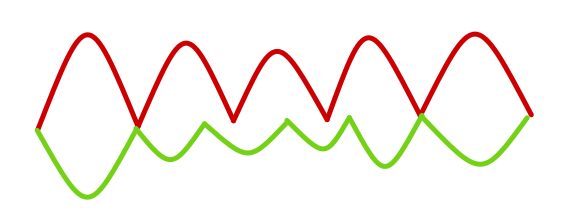
\includegraphics[scale=0.2]{picture/pic1.png}
\end{center}
注意到 $y_{1 \sim p+1}$ 和 $y_{2 \sim p+2}$ 分别是 $1 \rightarrow y_{p+1}$ 和 $y_2 \rightarrow n$ 的长度 $p$ 的最短路,所以把它们分别与 $\{x\}$ 应用路径单调性即得定理。
\end{frame}
\begin{frame}{回到例题 2——路径单调性应用}
	先以某个村庄断环成链,然后将这个链向右复制一份。设断环成链坐标是 $0$,先 $O(n \log V)$ 跑出 $0 \rightarrow L$ 长度为 $k$ 的字典序最小的最短路 $x_1=0,x_2,\cdots,x_{k+1}=L$。
	
	~\\
	
	设全局字典序最小的最短路是 $y_1\in[0,L),y_2,\cdots,y_{k+1}=y_1+L$,那么 $y_k-L,y_1,y_2,\cdots,y_k$ 也是 $y_k-L$ 到 $y_k$ 的最短路。由这两个序列与 $x$ 序列的关系,有 $\forall i\in[1,k],y_i \in [x_i,x_{i+1}]$,也就是说存在最优解每段里恰好经过一个节点。这样可以任选一段枚举其中所有村庄断环成链计算答案。
	
	选择 $[x_i,x_{i+1}]$ 中村庄数量最少的,村庄数量为 $O(\frac{n}{k})$。每次运行 $O(nk)$ 的动态规划,复杂度 $O(n^2)$,去掉一个 $\log$ 但还不够。
\end{frame}
\begin{frame}{加大力度——拓展分治解决决策单调性}
	上面的讨论给出了以下两个结论:
	\begin{enumerate}
		\item 最优解选的字典序最小的序列 $y_1 < y_2 < \cdots<y_k$ 有 $y_i \in [x_i,x_{i+1}]$,其中 $x_1=0,\cdots,x_{k+1}=L$ 是断环成链后跑 $0 \rightarrow L$ 的最小字典序最短路序列;
		\item 不妨设 $y_1 \in [x_1,x_2]$,跑出 $y_1 \rightarrow y_1+L$ 的最短路答案序列是 $y_1<y_2<\cdots<y_{k+1}=y_1+L$,则 $y_1$ 增大时 $y_i(i \in [1,k+1])$ 不会变小,这由路径单调性直接得出。
	\end{enumerate}
	利用 2 的单调性可以对分治算法进行拓展加速计算:设 \texttt{solve($l_1,r_1,l_2,r_2,\cdots,l_k,r_k$)} 表示计算 $k$ 个断点各自的范围内的最优解,每次取 $[l_1,r_1]$ 的中点作为第一个断点,然后做 $k-1$ 次 SMAWK 计算选 $k$ 个断点的最优解和方案,然后将 $k$ 个区间都劈开分治下去。
\end{frame}
\begin{frame}{最后一步——复杂度分析}
	单层分治复杂度 $O(\sum r_k-l_k)$,这就是 $O(n(\log n + \log V))$ 算法!别急,其实这个算法现在是 $O(nk)$ 的。\pause
	
	这其实是很好理解的,分治区间长度至多是 $O(n)$,每个区间至少需要 $O(k)$ 的操作,所以至少是 $O(nk)$ 的。
	
	产生这个问题的根本原因是该分治相比于普通分治,分治中点同时分到了两个区间里面。\pause
	
	优化很显然,由于最短区间长度是 $O(\frac{n}{k})$ 的,把这个区间转到第一个区间做,复杂度就正确了。
	
	同时这题时限大,所以可以把 Wilber 和 SMAWK 分别换成好写的二分栈和分治,这样每个过程的复杂度都乘个 $\log n$,也就是 $O(n \log n(\log n + \log V))$。
\end{frame}
\section{四边形不等式的其他应用}
\subsection{蒙日阵的生成}
\begin{frame}{蒙日阵的性质}
	这部分简要探讨一下如何生成一个随机性较强的蒙日阵。可以发现当矩阵 $C,D$ 是蒙日阵时,以下矩阵均是蒙日阵:
	\begin{enumerate}
		\item $C+D$;
		\item $\lambda C$,其中 $\lambda \geq 0$;
		\item $C^T$。
	\end{enumerate} 
	因此可以使用若干常见的蒙日阵进行随机线性组合得到随机性较强的蒙日阵。
\end{frame}
\begin{frame}{常见的简单蒙日阵}
	这里举若干常见的简单蒙日阵例子,假设蒙日阵大小为 $n \times m$;
	\begin{enumerate}
		\item 你所见到的所有决策单调性 DP 题目里的权矩阵;
		\item $a_{x,y} = \min(x,y)$;
		\item $a_{x,y} = \max(x,y)$;
		\item $a_{x,y}=xy$;
		\item $a_{x,y} = |x-y|^p$,$p \geq 1$;
		\item $a_{x,y} = \sum_{i=1}^x \sum_{j=y}^m d_{i,j}$,其中矩阵 $\{d_{i,j}\}$ 是一个 $n \times m$ 的非负元素矩阵;
		\item $a_{x,y} = [x=k]v_k$。
		\item $a_{x,y} = f(x-y)$,其中 $f(x)$ 是下凸函数。
	\end{enumerate}
\end{frame}
\begin{frame}{蒙日阵与次模函数}
	\begin{definition}[次模函数]
		对于有限集合 $E$ 和定义在幂集 $2^E$ 上的实函数 $f$,当且仅当对于任意 $X,Y \subseteq E$ 有 $f(X)+f(Y) \geq f(X \cap Y) + f(X \cup Y)$ 时称 $f$ 为\textbf{次模函数(submodular function)}。
	\end{definition}
	给出定义在集合 $E$ 上的次模函数 $f$ 和由 $E$ 中元素构成的排列 $d_1,\cdots,d_{|E|}$,考察 $|E| \times |E|$ 矩阵 $f$:
	
	$$f_{i,j} = \begin{cases}
	+\infty, & i > j \\
	-f(\{d_i,d_{i+1},\cdots,d_j\}),& i \leq j
	\end{cases}$$
	容易证明它满足四边形不等式。例题 1 里的斯坦纳树边数就是满足该性质的函数。
\end{frame}
\begin{frame}{次模函数举例}
	可以用次模函数来构造蒙日阵:
	\begin{enumerate}
		\item 拟阵的秩函数是次模函数(2018 论文),所以 $E$ 取拟阵全集,$f(X)$ 取拟阵秩函数值可以构造蒙日阵;
		\item 点集的割权函数是次模函数(2016 论文),所以 $E$ 取点集,$f(X)$ 取将 $X$ 与其他点割开的割集边权和可以构造蒙日阵;
		\item 集合并函数是次模函数,所以取某个集合 $S$,$E \subseteq 2^S$,$f(X) = |\cup_{S \in X} S|$ 可以构造蒙日阵。斯坦纳树边数就属于这一类。
	\end{enumerate}
	当然还有很多其他次模函数,有兴趣的同学可自行研究。
\end{frame}
\subsection{*连续子矩阵最小值查询}
\begin{frame}{例题 3:连续子矩阵最小值查询}
	Source:没有
	
	\sout{来个 DS 题放松一下}
	
	给定一个 $n \times n$ 的蒙日阵 $A$,保证在 $O(n)$ 复杂度内预处理后可以 $O(1)$ 计算 $A$ 中任意元素取值。$q$ 次询问,每次给出 $l_1,r_1,l_2,r_2$,求 $A_{[l_1 \sim r_1],[l_2 \sim r_2]}$ 的最小值。$n,q \leq 10^5$
\end{frame}
\begin{frame}{子问题——子列最小值查询}
	二维线段树预处理 $O(n^2)$ 不优秀。
	
	考虑先解决 $l_2=r_2$ 的子问题。对行建立线段树,每个行区间处理出这个行区间内每列的最小值所在位置。直接维护信息量 $O(n^2)$ 无法接受,但 $A_{[l,r],[1,n]}^T$ 是蒙日阵所以列最小值位置是单调的,即可将列划分为 $O(r-l)$ 个区间,每个区间内最小值所在行相同。维护这些区间信息量降低为 $O(n \log n)$。\pause
	
	考虑如何从左右儿子合并计算出当前节点答案。由于列最小值单调,所以列最小值位置序列的某段前缀由左儿子复制来,剩余一段由右儿子后缀复制来。二分找到分界点之后复制区间即可。预处理复杂度 $O(n \log n)$。
	
	询问时找到 $[l_1,r_1]$ 在线段树上的区间定位然后二分找到每个行区间在 $l_2$ 列上的最小值,单次询问复杂度 $O(\log^2 n)$。用分散层叠优化掉一个 $\log$ 变为单次 $O(\log n)$ 查询。
\end{frame}
\begin{frame}{子矩阵查询}
	对输入矩阵转置后该算法可以 $O(\log n)$ 查询 $l_1=r_1$ 时的最小值。
	
	对行建立线段树并维护列最小值位置区间。对于每个线段树节点 $[l,r]$,假设第 $l \leq i \leq r$ 行作为 第 $L_i$ 到 $R_i$ 列的列最小值位置,则计算 $v_i$ 表示 $A_{[i \sim i],[L_i \sim R_i]}$ 的最小值。由于从左右儿子合并只有 $O(1)$ 段产生变化,故只需要询问 $O(n)$ 次子行最小值。然后每个节点对 $v_i(l \leq i \leq r)$ 建立线段树。这部分复杂度 $O(n \log n)$。
	
	查询时先在行线段树上定位出 $\log n$ 个区间。那么在每个区间中需要计算出 $l_2 \sim r_2$ 这些列的列最小值的最小值。二分求出第 $l_2$ 列最小值在行 $p$、第 $r_2$ 列最小值在行 $q$,若 $p=q$ 则转化为一次行最小值,否则转化为求 $v_{p+1 \sim q-1}$ 的最小值和两次行最小值。查询复杂度 $O(\log^2 n)$。
	
	实际上该问题已有更优做法,可 $O(n)$ 预处理 $O(\log n)$ 完成子矩阵查询,但需要 $O(n)-O(1)$ rmq 之类的东西所以略过。
\end{frame}
\subsection{旅行商问题}
\begin{frame}{例题 4:挑战旅行商}
	Source:没有
	
	给定一个 $n \times n$ 的蒙日阵 $A$,保证对角线元素全 $0$,保证在 $O(n)$ 复杂度内预处理后可以 $O(1)$ 计算 $A$ 中任意元素取值。求以该矩阵为邻接矩阵的带权有向图中边权和最小的经过所有点恰好一次的回路。$n \leq 10^6$
\end{frame}
\begin{frame}{双调回路}
	\begin{definition}[双调回路]
		对于带权有向图 $G$,定义图上按照 $1<i_1<i_2<\cdots<i_{k_1}<n>j_1>j_2>\cdots>j_{k_2}>1$ 顺序经过所有节点恰好一次的回路为图 $G$ 上的一条\textbf{双调回路(pyramidral tour)}。
	\end{definition}
	任意哈密顿路的边权和最小值不容易计算,但是容易设计一个动态规划来计算一张图上双调回路的边权和最小值:设 $f_{i,j}$ 表示形如 $i>p_1>p_2>\cdots>1<q_1<q_2<\cdots<q_k<j$ 的路径的边权最小值,转移根据 $i,j$ 的差值关系枚举 $p_1$ 或 $q_k$ 转移,只有当 $|i-j|=1$ 时需要枚举前驱,其他情况前驱是确定的,复杂度 $O(n^2)$。
\end{frame}
\begin{frame}{蒙日阵与双调回路}
	\begin{theorem}
		当带权有向图 $G$ 的邻接矩阵是蒙日阵时,存在旅行商问题的一个解回路是双调回路。
	\end{theorem}\pause
	对点数 $n$ 归纳:$n \leq 3$ 时所有回路都是双调回路;结论对 $n-1$ 成立时,考察某个不是双调回路的最优回路,其存在某点 $p$ 满足前驱 $pre_p < p$ 且后继 $suf_p < p$。由四边形不等式 $w_{pre_p,suf_p}+w_{p,p} \leq w_{pre_p,p}+w_{p,suf_p}$,所以把 $p$ 拿出来 $pre_p$ 接 $suf_p$ 之后权值不会更大。此时图上有一个大小为 $n-1$ 的回路,考察其导出子图根据归纳假设换成最优双调回路答案不会变大。最后在回路上找到 $q$ 使得 $q<p<suf_q$,由四边形不等式 $w_{q,p}+w_{p,suf_q} \leq w_{p,p}+w_{q,suf_q}$,所以把 $p$ 插进去就得到了权值不比之前回路大的双调回路。
\end{frame}
\begin{frame}{优化双调回路计算}
	最优双调回路计算是 $O(n^2)$ 的,摆脱了指数级但不够优秀。
	
	把动态规划中有转移的 $O(n)$ 个状态拿出来。设 $F_i = f_{i+1,i},G_i = f_{i,i+1}$,答案是 $\min(F_{n-1}+w_{n-1,n},G_{n-1}+w_{n,n-1})$。转移枚举大一维的前驱:
	\begin{gather*}
		F_i = \min_{1 \leq j \leq i-1} G_j+w_{i+1,j}+\sum_{k=j+1}^{i-1}w_{k,k+1} \\
		G_i = \min_{1 \leq j \leq i-1} F_j+w_{j,i+1}+\sum_{k=j+1}^{i-1}w_{k+1,k}
	\end{gather*}
	这是交错型的动态规划。预处理前缀和之后转移权值可以 $O(1)$ 算出。
\end{frame}
\begin{frame}{优化双调回路计算}
	对于 $(n-1) \times (n-1)$ 的矩阵 $A$,即 $F$ 的转移矩阵,$$a_{j,i} = \begin{cases}
	+\infty, &j\geq i\\
	w_{i+1,j}+\sum_{k=j+1}^{i-1}w_{k,k+1}, & j<i
	\end{cases}$$考虑证明它是蒙日阵,即计算 $a_{j,i}+a_{j+1,i+1}-(a_{j,i+1}+a_{j+1,i})$ 的值并比较它和 $0$ 的大小关系。$G$ 的转移矩阵同理。
	
	求和部分转化为前缀和相减形式显然可以抵消,故 $a_{j,i}+a_{j+1,i+1}-a_{j,i+1}-a_{j+1,i}=w_{i+1,j}+w_{i+2,j+1}-w_{i+1,j+1}-w_{i+2,j} \leq 0$,这样 $F$ 的转移矩阵满足四边形不等式,$G$ 同理,因此使用二分栈或 Eppstein 算法加速决策单调性,复杂度 $O(n \log n)$ 或 $O(n)$。
\end{frame}
\section{}
\begin{frame}{End}
\begin{center}
\begin{huge}
Thanks for your listening!
\end{huge}
\end{center}
\end{frame}
\end{document}